%  $Description: Author guidelines and sample document in LaTeX 2.09$
%
%  $Author: ienne $
%  $Date: 1995/09/15 15:20:59 $
%  $Revision: 1.4 $
%
%\documentclass[times, 10pt,twocolumn]{article}
\documentclass[conference,final]{IEEEtran}
\usepackage{latex8}
\usepackage{times}

% Users' option
\usepackage{amssymb}
\usepackage{amsmath}
\usepackage{graphicx}
\usepackage{epstopdf}
\usepackage{color}
\topmargin=0.001in
\usepackage{multirow}
\usepackage{booktabs}
\newif\ifdraft
\drafttrue

\renewcommand{\multirowsetup}{\centering}
\renewcommand{\arraystretch}{1.2}
\def\nyc{\centering}

\ifdraft
\newcommand{\fixme}[1]{ { \bf{ ***FIXME: #1 }} }
\newcommand{\jhanote}[1]{ {\textcolor{red} { ***Jha: #1 }}}
\newcommand{\Nkimnote}[1]{ {\textcolor{green} { ***Nkim: #1 }}}
\newcommand{\skonote}[1]{ {\textcolor{blue} { ***Jeff: #1 }}}
\newcommand{\athotanote}[1]{ {\textcolor{green} { ***athota: #1 }}}
\newcommand{\Jkimnote}[1]{ {\textcolor{red} { ***Jkim: #1 }}}
\newcommand{\yyenote}[1]{ {\textcolor{blue} { ***yye00: #1 }}}
\else
\newcommand{\jhanote}[1]{}
\newcommand{\Nkimnote}[1]{}
\newcommand{\fixme}[1]{}
\newcommand{\skonote}[1]{}
\newcommand{\Jkimnote}[1]{}
\fi
% End of users' option

%\documentstyle[times,art10,twocolumn,latex8]{article}

%-------------------------------------------------------------------------
% take the % away on next line to produce the final camera-ready version
\pagestyle{empty}

\newcommand{\up}{\vspace*{-1em}}
\newcommand{\upp}{\vspace*{-0.5em}}
\newcommand{\ts}{$T_{s}$}


%-------------------------------------------------------------------------
\title{A Hybrid CFD-MD Simulation Framework with Coscheduling and Load Balancing}

\author{
 ~\\[-2em]
 Soon-Heum Ko$^{1}$, Nayong Kim$^{1}$, Abhinav Thota$^{1,2}$ (?), \\
 Dimitris Nikitopoulos$^{3}$, Dorel Moldovan$^{3}$ (?), Shantenu Jha$^{*1,2}$\\
 \small{\emph{$^{1}$Center for Computation \& Technology, Louisiana State University, USA}}\\
 \small{\emph{$^{2}$Department of Computer Science, Louisiana State University, USA}}\\
 \small{\emph{$^{3}$Department of Mechanical Engineering, Louisiana State University, USA}}\\
 \small{\emph{$^{*}$Contact Author}}\\
}

%\thispagestyle{empty}

\begin{document}


\maketitle

\begin{abstract}

\skonote{Title needs change}

 Something
\end{abstract}
\up\up


%-------------------------------------------------------------------------
\section{Introduction and Motivation}


The need for accurately solving micro/nanoscale flow field is increasing these days with more invent (or design/development) of biofluidic systems.\\
\skonote{Necessity of solving micro/nanoflow: 1 Paragraph}
\newline
\newline


A hybrid CFD-MD approach is a modern numerical technique to resolve the micro/nanofluid flow satisfying both accuracy and efficiency.\\
\skonote{Briefly introducing the hybrid CFD-MD: advantages from the problems in conventional CFD and MD: 1 Paragraph}
\newline
\newline


Severals of numerical researches have been performed in developing/improving numerical techniques for the hybrid CFD-MD simulation or figuring out the flow physics in nano-scale systems.~\cite{Thompson},~\cite{Nie},~\cite{Yen},~\cite{Steijl},~\cite{Kotsalis}\\
\skonote{About the previous works: 2 Paragraphs}
\newline
\newline


Though much improvement have been made on developing numerical techniques for the hybrid CFD-MD simulation, still a lot of issues are raised on refining the hybrid CFD-MD scheme.\\
\skonote{Raise the issue and our focus of parametric study: 1 paragraph}
\newline
\newline


Meanwhile, integrating two (or more) application domains for a multi-physics research raises another issue in view of computational science: how to couple two independent software packages from different disciplines and control/manage the operation flow of separate codes within the computer systems.\\
\skonote{Issues of coupling on supercomputers: coscheduling and load balancing. 1 paragraph}
\newline
\newline


Conceptually, the adoption of a container job can be an answer to resolve the coscheduling and load balancing issues of running a coupled multi-task simulation.\\
\skonote{Introduce container job and related researches from other researchers: show their limitation as well - i.e., LB issue, etc.. Include REMD, co-scheduling of multiple tasks via SGE in Ranger. 2 paragraphs}
\newline
\newline


Collectively, we are focusing on investigating numerical issues of applying the hybrid CFD-MD scheme to a nanofluidic system, as well as designing and developing an efficient runtime framework for a coupled multi-component simulation.\\
\skonote{Tell the objectives of this research: Develop a Hybrid CFD/MD Simulation Framework including Domain Science Application Codes and Computational Framework. Mention that 'we basically used an in-house CFD code and famous LAMMPS MD package and modified both codes for coupled multi-physics simulation. We focus more on building an efficient coupled multi-task environment for hybrid CFD-MD simulation.' Also include the composition of chapters in the follow. 2 paragraphs}
\newline
\newline


% -------------------------------------------------------------------------
\section{A Hybrid CFD-MD Simulation Approach}


\subsection{Macroscopic Flow Characteristics by Continuum Hypothesis}


CFD simulations are mostly the procedure of numerically solving Navier-Stokes equations, which is the formulation of Newton's second law to a sufficiently large flow system where the continuum hypothesis is commonly accepted.\\
\skonote{Brief Introduction of CFD: 1 paragraph. What is continuum hypothesis and how small is the acceptable range.}
\newline
\newline


In this research, we have based on the ``in-house'' incompressible CFD code~\cite{Lee} as the CFD component for the coupled simulation.\\
\skonote{Features of a CFD Code: Governing equations and discretization / numerical methods. 2-3 paragraphs. Also mention that the code is ''parallelized'' and additional implementation of coupling scheme on CFD part has been done, which is to be discussed in the below.}
\newline
\newline


\subsection{Detailed Flow Simulation with Intermolecular Effect}


What is MD? by Nayong\\
\skonote{Brief Introduction of MD}
\newline
\newline


Governing equations, numerical schemes inside: by Nayong\\
\skonote{Features of an MD Code: Governing equations with force field/ numerical methods}
\newline
\newline


\subsection{Implementation of Hybrid Schemes}


The hybrid CFD-MD approach basically starts from the concept that the intertial force dominates the system while intermolecular effect cannot be negligible in the low-speed flow region. As given in Fig.~\ref{Fig:CFD-MD_Schematic}-(a), CFD approach analyzes the macroscopic flow characteristics with the moderate flow velocity, while MD independently solves low-speed flow region. These two domains overlap in the middle, where CFD and MD exchange their solutions.\\
\skonote{How to Couple: Schematic of CFD and MD zones. 1 paragraph.}
\newline
\newline


%%%%% FIGURE %%%%%
\begin{figure}
\centering
\includegraphics[scale=0.3]{CFD-MD_Schematic_a.eps}
\linebreak
\includegraphics[scale=0.3]{CFD-MD_Schematic_b.eps}
\caption{\small Title: CFD-MD Schematic}
\label{Fig:CFD-MD_Schematic}
\vspace{-1em}
\end{figure}
%%%%% FIGURE %%%%%


The overlap region can be divided to five layers, as given in Fig.~\ref{Fig:CFD-MD_Schematic}-(b).\\
\skonote{Meaning of each layer within overlap region. 1 paragraph.}
\newline
\newline


In detail, different numerical modelings are applied on these layers.\\
\skonote{Numerical modeling and implementation on each solver. 3 paragraphs. Start with external force layer: specify the equation, mention that 'this artificial force modeling is implemented on MD package, to trap escaping particles within the computational domain'. Next paragraph about CFDtoMD: Discuss the meaning of constrained MD equation and specify how the code is changed, mention that 'this constrained MD equation specifies that particles in this layer eventually follow the averaged flow speed from the continuum approach.' Last paragraph about MDtoCFD: express that the average of particle velocity in this layer is applied to CFD's boundary condition, changing the CFD code.}
\newline
\newline


Figure ~\ref{Fig:Code_Flowchart} expresses the coupled simulation flow.\\
\skonote{Explain the flow of each simulation code in detail. Mention about when and where the data exchange takes place: if needed, have additional figure to explain data exchange interval with the evolution timeline. Mention also which data to exchange. Mention that 'we currently adopt the file-based data exchange mechanism.' 2 paragraphs.}
\newline
\newline


%%%%% FIGURE %%%%%
\begin{figure}
\centering
\includegraphics[scale=0.3]{Code_Flowchart.eps}
\caption{\small Title: Flowchart of Codes}
\label{Fig:Code_Flowchart}
\vspace{-1em}
\end{figure}
%%%%% FIGURE %%%%%


\subsection{Numerical Result of a Nano-scale Couette Flow Simulation}


The geometry of a nano-scale channel along with the size of each domain is given in Fig.~\ref{Fig:Channel_Mesh}.\\
\skonote{Description of a problem: 1 paragraph. Include size of each domain, layers in hybrid region, velocity of an upper wall.}
\newline
\newline


%%%%% FIGURE %%%%%
\begin{figure}
\centering
\includegraphics[scale=0.3]{Channel_Mesh.eps}
\caption{\small Title: Channel System}
\label{Fig:Channel_Mesh}
\vspace{-1em}
\end{figure}
%%%%% FIGURE %%%%%


The result of a Couette flow in this channel is shown in Fig.~\ref{Fig:Solution_Couette}.\\
\skonote{Solution of Couette Flow: Compare the result with pure CFD, pure MD and Nie��s work. Also discuss the limit of current simulation in the next paragraph: it's an unrealistic simulation, algorithms and models are still improving (like governing equations in CFD - secondary flow, flux scheme for low speed flow, artificial external force in hybrid region) Totally 2 paragraphs.}
\newline
\newline


%%%%% FIGURE %%%%%
\begin{figure}
\centering
\includegraphics[scale=0.3]{Solution_Couette.eps}
\caption{\small Title: Couette Flow Solution}
\label{Fig:Solution_Couette}
\vspace{-1em}
\end{figure}
%%%%% FIGURE %%%%%


Parametric study or unsteady simulation result to be included here\\
\skonote{1-2 paragraphs.\\
Parametric Study of (choose one of the following issues for more numerical results)\\
a. Domain Size (CFD/MD/Hybrid) for Solution��s Accuracy and Efficiency\\
b. Layer Size (CFD/MD) and Its Position, Imposing the Velocity via Function\\
c. Sampling (Averaging) Time Scale and Its Interval}
\newline
\newline


%-------------------------------------------------------------------------
\section{Construction of a Coupled Multi-physics Simulation Framework with Co-scheduling and Load Balancing}
\subsection{SAGA and SAGA-based Frameworks for Coupled Multi-component Computations}


\skonote{Refer to Section 3 in CCGrid2010.}
\newline
\newline


%\section{SAGA and SAGA-based Frameworks for Large-Scale and Distributed Computation}

% The Simple API for Grid Applications (SAGA) is an API standardization effort within the Open Grid Forum (OGF)~\cite{ogf_web}, an international standards development body concerned primarily with standards for distributed computing. SAGA provides a simple, POSIX-style API to the most common Grid functions at a sufficiently high-level of abstraction so as to be independent of the diverse and dynamic Grid environments. The SAGA specification defines interfaces for the most common Grid-programming functions grouped as a set of functional packages (Fig.~\ref{Fig:SAGA1}). Some key packages are:


\begin{figure}
 \begin{center}
     \includegraphics[width=0.40\textwidth]{stci_saga_figures-1.eps}
 \end{center}
\caption{\small Layered schematic of the different components of the SAGA landscape. At the topmost level is the simple integrated API which provides the basic functionality for distributed computing. Our BigJob abstraction is built upon this SAGA layer using Python API wrapper}
 \label{Fig:SAGA1}
 \vspace{-1em}
\end{figure}


%\begin{itemize}
%\item File package - provides methods for accessing local and remote filesystems, browsing directories, moving, copying, and deleting files, setting access permissions, as well as zero-copy reading and writing
%\item Job package - provides methods for describing, submitting, monitoring, and controlling local and remote jobs. Many parts of this package were derived from the largely adopted DRMAA % ~\cite{drmaa_url} specification.
%\item Stream package - provides methods for authenticated local and remote socket connections with hooks to support authorization and encryption schemes.
%\item Other Packages, such as the RPC (remote procedure call) and Replica package
%\end{itemize}


\skonote{Exclude the mention about the multiple BigJobs. Also, focus on explaining BigJob's advert service module in detail, including referring to Andre's paper}
\newline
\newline


% Fig.~\ref{Fig:BigJob_Structure} shows the structure of BigJob and its operation flow. When a BigJob is submitted to the remote resource, the application manager monitors the status of this pilot-job through the advert service. When resources are allocated to the BigJob, the application manager allots the obtained resources to its sub-jobs and a coupled simulation starts under the control of a multi-physics agent in the remote resource. Advert service keeps on getting the status of a pilot-job from the queuing system and the status of sub-jobs from multi-physics agent and also delivers this information to the application manager by a push-pull mechanism. The application manager watches the status of sub-jobs and decides the next event when the coupled simulation is finished. When one default BigJob is launched, sub-jobs keeps running until final solution is achieved and the manager quits the Pilot-Job at that time. In case multiple BigJobs are submitted for the same simulation or if a load balancing function is included, sub-jobs experience several restarts from their checkpointing data, reflecting changed processor allocation to each application. In the former case, resource allocation to each sub-job follows a pre-defined map according to the number of BigJobs allotted to the simulation; in the latter case, resource allocation to each sub-job becomes dynamic according to its performance, as discussed in the next section.

%%%%% FIGURE %%%%%
\begin{figure}
\centering
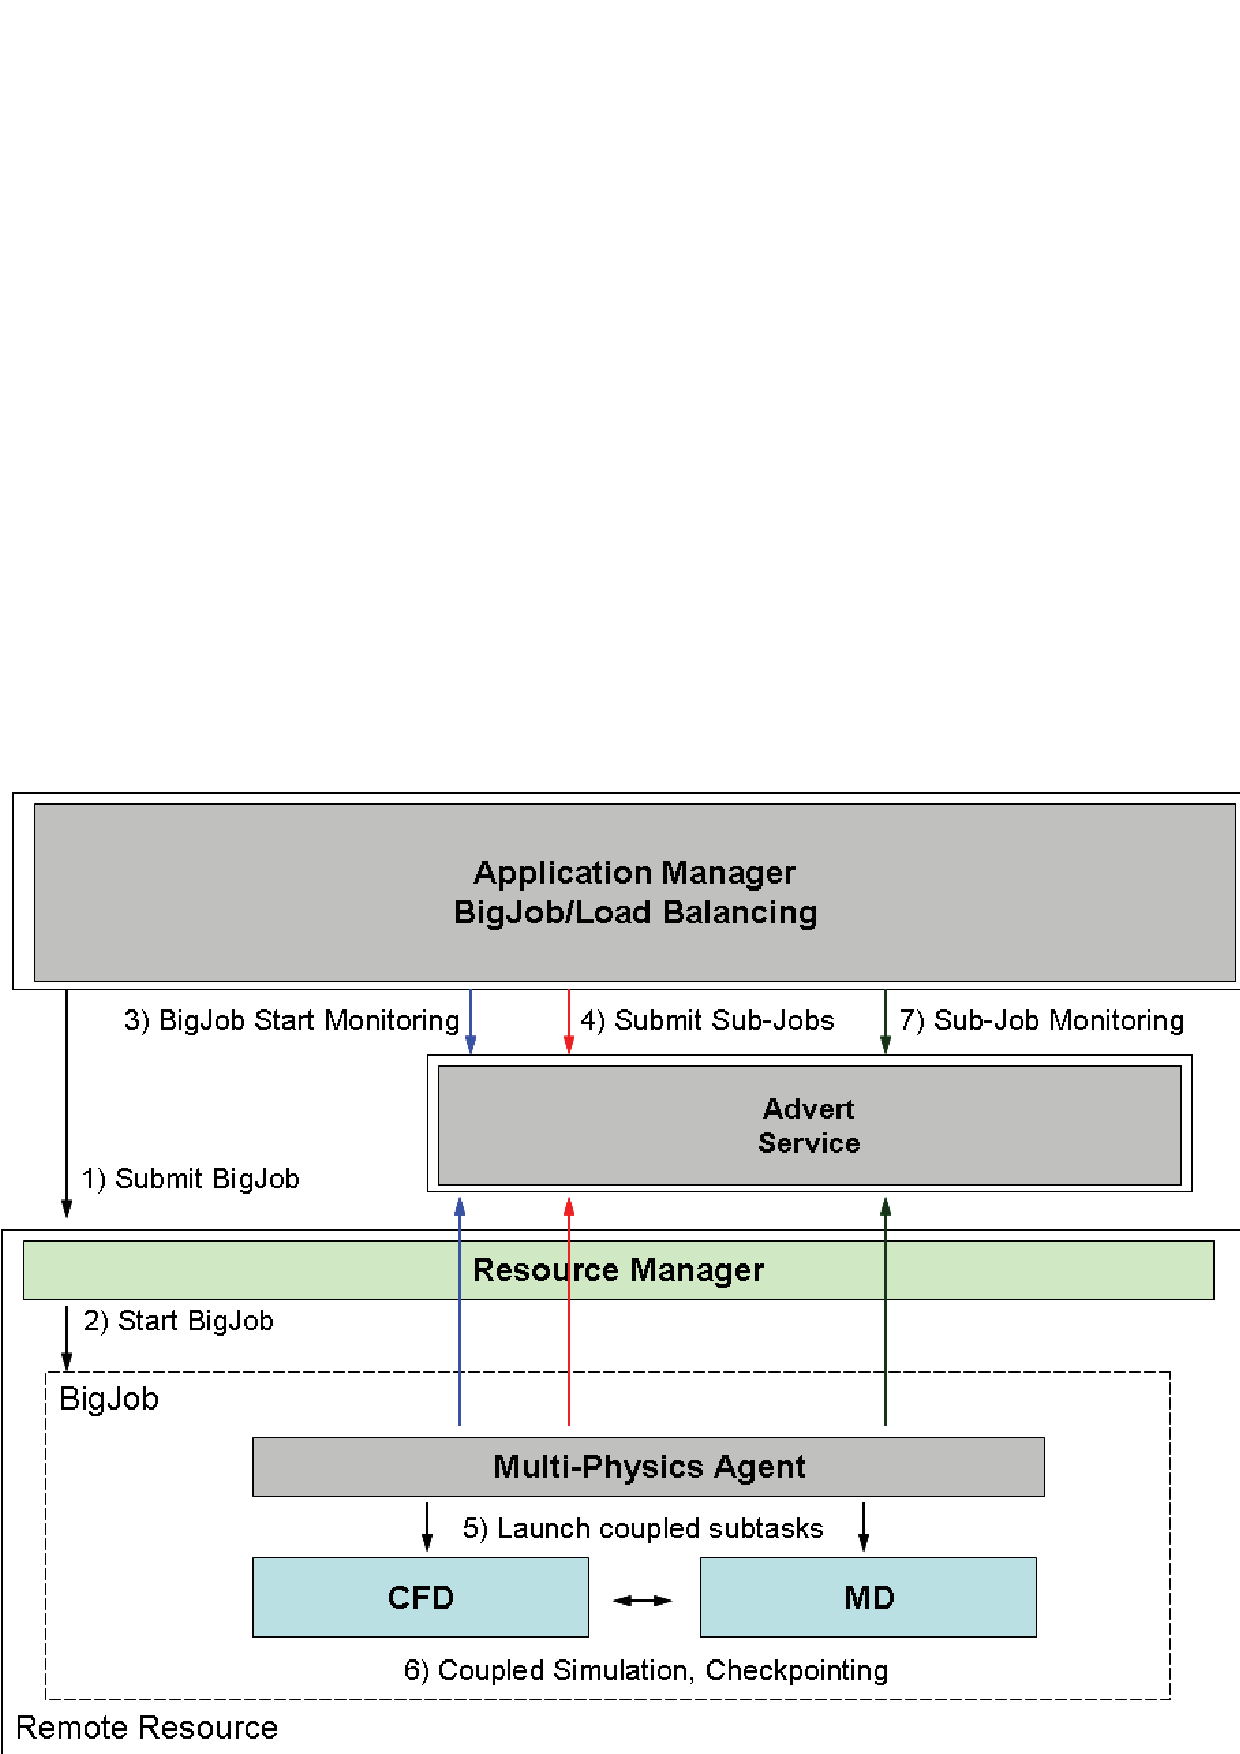
\includegraphics[scale=0.38]{Structure_of_BigJob}
\caption{\small Architecture of the Controller/Manager and Control Flow: Application manager is responsible for job management including BigJob and sub-job submission, their status monitoring functions. We implement a load balancing module, and migration service based on job information. Application agent system resides on each HPC resource and conducts job information gathering and also communicates with the application manager via the advert service}
\label{Fig:BigJob_Structure}
\vspace{-1em}
\end{figure}
%%%%% FIGURE %%%%%


\subsection{Load Balancing for Coupled Multi-Physics Simulation}


\skonote{Based on Section 4 in CCGrid 2010: Refine LB, include motivation etc. (e.g., Not touching application codes)}
\newline
\newline


%\section{Load Balancing for Coupled Multi-Physics Simulation}

% The flexibility to re-distribute resources (processors) to the individual task does not imply efficient utilization. This is the responsibility of a load-balancer (LB). We will discuss the implementation and algorithm of this LB~\cite{Ko}; it is important to mention that the LB functions in the context of the SAGA-BigJob framework.
% Each application's load is determined by its elapsed time to run the evolution loop. Here, time for initialization or inter-domain data exchange are excluded from the counting, because they are one-time events or irrelevant to application's performance.  The efficient functioning of the LB is predicated on application codes being able to restart from their checkpointing data effectively.  Also, application codes should be equipped with generalized domain partitioning routine to run a simulation with any number of processors, without harming their parallel efficiency a lot. If above conditions are satisfied, it makes sense to load the LB within the pilot-job, to implement dynamic resource allocation between tasks.  Conceptually, the load-balancing algorithm assigns more processors to a sub-task with greater runtime, until the two codes take the same wall-clock time between points when they communicate.
% Interestingly, our approach is very simple and the algorithm is indepenendent of applications upon the predications of,
%(1) each application code follows the ideal parallel efficiency.
%(2) all processors in one node are assigned to one single task.

%Let the computation time (between exchanges) of the two sub-jobs be $t_{CFD}$ and $t_{MD}$, and the number of processors assigned to each domain be $PE_{CFD}$ and $PE_{MD}$, respectively. Subscripts I and F denotes initial and final states. Based on assumption (1), total problem size of each application remains the same after resource re-allocation,

%\vspace{-.2em}
%\footnotesize
%\begin{eqnarray}
%W_{CFD}&=&PE_{CFD,I}\times t_{CFD,I}=PE_{CFD,F}\times t_{CFD,F} \nonumber \\
%W_{MD}&=&PE_{MD,I}\times t_{MD,I}=PE_{MD,F}\times t_{MD,F}
%\label{eq:SimTime_EachTask}
%\end{eqnarray}
%\normalsize

% In spite of the re-allocation, the total number of processors utilized remains the same:

%\vspace{-.2em}
%\footnotesize
%\begin{equation}
%PE_{TOT}=PE_{CFD,I}+PE_{MD,I}=PE_{CFD,F}+PE_{MD,F}
%\label{eq:PECondition}
%\end{equation}
%\normalsize

% Our objective is to reduce the computation time of a sub-job to the point until the two application components show the same computation between the exchange points, i.e., $t_{CFD,F} = t_{MD,F}$. From Equation~\ref{eq:SimTime_EachTask} and Equation~\ref{eq:PECondition} an optimal number of processors distributed for the CFD subtask would be:

%\vspace{-.2em}
%\footnotesize
%\begin{eqnarray}
%PE_{CFD,F} & = & \frac {W_{CFD}} {(W_{CFD} + W_{MD})} \times PE_{TOT}
%\end{eqnarray}
%\normalsize

% The MD simulation (sub-job) will follow a similar expression. The optimal processor distribution from above equation will return a non-integer value. Also, under the second assumption (which is the policy of many supercomputing centers), any load-balancing determined as above, will proceed in discrete values expressed as the multiples of the number of CPU cores in a node. We choose the nearest discrete number to our load balancing as the optimal number of processor on each application.


\subsection{Implementation of an Execution Framework to Support Multi-physics Applications}


\skonote{Refer to Section 5.a in CCGrid 2010}
\newline
\newline


The application manager along with its load balancing functionality is implemented as follows.\\
\skonote{Features of an application manager: Mention that it is written in PYTHON, load balancing function is implemented inside, etc. 1 paragraph}
\newline
\newline


To use the BigJob and its load balancing function, application codes also need minor modifications.\\
\skonote{Changes of Application Codes. 1 paragraph}
\newline
\newline


The generation of an application manager and the changes in application codes raise the possible simulation scenarios as given in Fig.~\ref{Fig:OneBJ_Flow}.\\
\skonote{Explain S1 and S1-LB scenarios. Just copy from Section 5.a in CCGrid 2010}
\newline
\newline


%%%%% FIGURE %%%%%
\begin{figure}
%\vspace{-1em}
\centering
\includegraphics[scale=0.4]{Simulation_Time_of_One_BigJob.eps}
\caption{\small Comparison of dependencies encountered for coupled
  simulations submitted as conventional jobs, to the scenario when
  using Pilot-Jobs. Here we use only 1 BigJob (S1). The conventional
  mode of submission experiences three phases based upon their queue
  state: (i) All jobs are waiting: ($t_1-t_0$); (ii) Inactive mode
  (where one job is waiting for another: $t_2-t_1$), and (iii) Active
  mode (running a coupled simulation: $t_f-t_2$). The Inactive stage,
  disappears when a coupled simulation runs within a BigJob, as an
  allocated BigJob distributes its resource to both sub-jobs.}
\label{Fig:OneBJ_Flow}
\vspace{-1em}
\end{figure}
%%%%% FIGURE %%%%%


\subsection{Performance Analysis of a Multi-physics Simulation Framework}


\skonote{Refer to Section 5.b and 5.c in CCGrid 2010}
\newline
\newline


The benefit of a BigJob as a way of reducing the waiting time on the local queueing system can be discussed from our preliminary test of the relationship between the requested number of processors and the waiting time.\\
\skonote{Queue Wait Time Analysis: Preliminary Test. Waiting Time with Different PX Requests, Wall Time Limit
(Mention that BQP is not perfect, especially measuring inactive waiting time of ��TWO CONVENTIONAL JOBS��). Include Table 1 here.\\
More test needed: Submit 128, 256 and 512 PX jobs with 6, 24, 48 wall limit times synchronously - to satisfy the same condition among testsuites. Also include BQP test at the same condition.}
\newline
\newline


A BigJob submission shows the saving of waiting time on the queue, not only the bigger job size has the higher priority in the queueing system but also one BigJob submission eliminates the inactive idling time of first allocated job in conventional job submission.\\
\skonote{Queue Wait Time Analysis: Waiting time of a BigJob and two conventional jobs. Emphasize the inactive time as well - it makes the conventional job submission to have longer wall time limit and it will even reduce the possibility of getting the backfilling capability. Include Table 2 here.\\
More test needed: One BigJob and two conventional jobs at 2-3 locations, with 3 PX settings (128,256,512) and 3 wall time limit (6,24,48)\\
  1. BigJob��s Faster Start by Queuing Policy\\
  2. Co-scheduling and the Safety: Different wall limit time between BigJob and Conventional Jobs due to Highly Unpredictable Inactive Time}
\newline
\newline


The simulation runtime with/without a BigJob is given in table 3.\\
\skonote{Runtime Analysis: Comparison of LB with conventional simulation time: different system size (with different ratio between CFD and MD), different number of simulation loop and different interval of simulation loop. Table 3 with 2 graphs - change of CPU allocation to each subjob with iteration time in 2 simulation cases.}
\newline
\newline


%-------------------------------------------------------------------------
\section{Next Step: Further Refinement}


%-------------------------------------------------------------------------
\section{Conclusions}



\section*{Acknowledgment}
This work is part of the Cybertools (http://cybertools .loni.org)
project and primarily funded by NSF/LEQSF (2007-10)-CyberRII-01.
Important funding for SAGA has been provided by the UK EPSRC grant
number GR/D0766171/1 (via OMII-UK). This work has also been made
possible thanks to computer resources provided by LONI. We thank Andre
Luckow for initial work on BigJob, Lukasz Lacinski for help with SAGA
deployment (via HPCOPS NSF-OCI 0710874) and Joao Abecasis for his work
on the SAGA Condor adaptors.

%-------------------------------------------------------------------------
%\nocite{ex1,ex2}
%\bibliographystyle{IEEEtran}
%\bibliography{saga_tg08}


\end{document}


